\documentclass[12pt,a4paper]{article}
\usepackage[utf8]{utf8}
\usepackage[margin=1in]{geometry}
\usepackage{tcolorbox}
\usepackage{tikz}
\usetikzlibrary{shapes.geometric, arrows.meta, positioning}

\title{\textbf{5. The Adventure}\\[0.3em] \Large Textbook Page 45}
\author{\textbf{Author:} Jayant Narlikar \quad|\quad \textbf{Textbook:} Hornbill (Class 11)}
\date{}

\begin{document}

\maketitle

\begin{tcolorbox}[colback=gray!5!white,colframe=gray!75!black,title=\textbf{Notice these expressions in the text. Infer their meaning from the context.}]
\begin{itemize}
    \item blow-by-blow account
    \item morale booster
    \item relegated to
    \item political acumen
    \item de facto
    \item astute
    \item doctored accounts
    \item gave vent to
\end{itemize}
\end{tcolorbox}

\vspace{0.5cm}

THE Jijamata Express sped along the Pune-Bombay\footnote{Now known as Mumbai} route considerably faster than the Deccan Queen. There were no industrial townships outside Pune. The first stop, Lonavala, came in 40 minutes. The ghat section that followed was no different from what he knew. The train stopped at Karjat only briefly and went on at even greater speed. It roared through Kalyan.

Meanwhile, the racing mind of Professor Gaitonde had arrived at a plan of action in Bombay. Indeed, as a historian he felt he should have thought of it sooner. He would go to a big library and browse through history books. That was the surest way of finding out how the present state of affairs was reached. He also planned eventually to return to Pune and have a long talk with Rajendra Deshpande, who would surely help him understand what had happened.

That is, assuming that in this world there existed someone called Rajendra Deshpande!

The train stopped beyond the long tunnel. It was a small station called Sarhad. An Anglo-Indian in uniform went through the train checking permits.

\vfill

\begin{figure}[htbp]
\centering
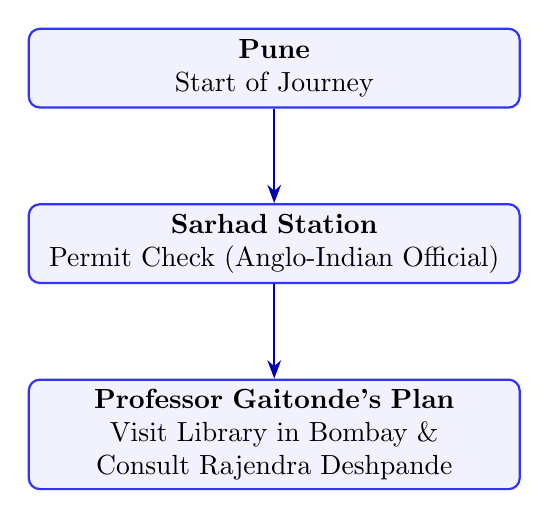
\begin{tikzpicture}[
    node distance=1.2cm,
    block/.style={rectangle, draw=blue!80, fill=blue!5, thick, rounded corners, text width=6cm, align=center, minimum height=1cm},
    arrow/.style={-Stealth, thick, draw=blue!70!black}
]
    \node[block] (pune) {\textbf{Pune}\\ Start of Journey};
    \node[block, below=of pune] (sarhad) {\textbf{Sarhad Station}\\ Permit Check (Anglo-Indian Official)};
    \node[block, below=of sarhad] (plan) {\textbf{Professor Gaitonde's Plan}\\ Visit Library in Bombay \& Consult Rajendra Deshpande};

    \draw[arrow] (pune) -- (sarhad);
    \draw[arrow] (sarhad) -- (plan);
\end{tikzpicture}
\caption{Page 1: Journey of Jijamata Express \& Gaitonde's Initial Plan}
\end{figure}

\end{document}
\documentclass[12pt,a4paper]{article}
\usepackage[utf8]{utf8}
\usepackage[margin=1in]{geometry}
\usepackage{tikz}
\usetikzlibrary{shapes.geometric, arrows.meta, positioning}

\title{\textbf{5. The Adventure}\\[0.3em] \Large Textbook Page 46}
\author{\textbf{Author:} Jayant Narlikar \quad|\quad \textbf{Textbook:} Hornbill (Class 11)}
\date{}

\begin{document}

\maketitle

"This is where the British Raj begins. You are going for the first time, I presume?" Khan Sahib asked.

"Yes." The reply was factually correct. Gangadharpant had not been to this Bombay before. He ventured a question: "And, Khan Sahib, how will you go to Peshawar?"

"This train goes to the Victoria Terminus\footnote{Now known as Chhatrapati Shivaji Terminus}. I will take the Frontier Mail tonight out of Central."

"How far does it go? By what route?"

"Bombay to Delhi, then to Lahore and then Peshawar. A long journey. I will reach Peshawar the day after tomorrow."

Thereafter, Khan Sahib spoke a lot about his business and Gangadharpant was a willing listener. For, in that way, he was able to get some flavour of life in this India that was so different.

The train now passed through the suburban rail traffic. The blue carriages carried the letters, GBMR, on the side.

"Greater Bombay Metropolitan Railway," explained Khan Sahib. "See the tiny Union Jack painted on each carriage? A gentle reminder that we are in British territory."

The train began to slow down beyond Dadar and stopped only at its destination, Victoria Terminus. The station looked remarkably neat and clean. The staff was mostly made up of Anglo-Indians and Parsees along with a handful of British officers.

As he emerged from the station, Gangadharpant found himself facing an imposing building. The letters on it proclaimed its identity to those who did not know this Bombay landmark:

\begin{center}
    \textbf{EAST INDIA HOUSE HEADQUARTERS OF\\ THE EAST INDIA COMPANY}
\end{center}

Prepared as he was for many shocks, Professor Gaitonde had not expected this. The East India Company had been wound up shortly after the events of 1857 --- at least, that is what history books said. Yet, here it was, not only alive but flourishing. So, history had taken a different turn, perhaps before 1857. How and when had it happened? He had to find out.

As he walked along Hornby Road, as it was called, he found a different set of shops and office buildings. There was no Handloom House building. Instead, there were Boots and Woolworth departmental stores, imposing offices of Lloyds, Barclays and other British banks, as in a typical high street of a town in England.

\vfill

\begin{figure}[htbp]
\centering
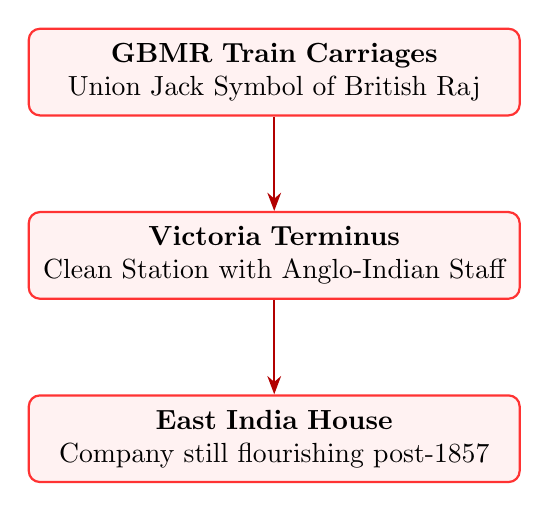
\begin{tikzpicture}[
    node distance=1.2cm,
    block/.style={rectangle, draw=red!80, fill=red!5, thick, rounded corners, text width=6cm, align=center, minimum height=1.1cm},
    arrow/.style={-Stealth, thick, draw=red!70!black}
]
    \node[block] (gbmr) {\textbf{GBMR Train Carriages}\\ Union Jack Symbol of British Raj};
    \node[block, below=of gbmr] (vt) {\textbf{Victoria Terminus}\\ Clean Station with Anglo-Indian Staff};
    \node[block, below=of vt] (eic) {\textbf{East India House}\\ Company still flourishing post-1857};

    \draw[arrow] (gbmr) -- (vt);
    \draw[arrow] (vt) -- (eic);
\end{tikzpicture}
\caption{Page 2: Key Indicators of British Rule in Alternate Bombay}
\end{figure}

\end{document}
\documentclass[12pt,a4paper]{article}
\usepackage[utf8]{utf8}
\usepackage[margin=1in]{geometry}
\usepackage{tikz}
\usetikzlibrary{shapes.geometric, arrows.meta, positioning}

\title{\textbf{5. The Adventure}\\[0.3em] \Large Textbook Page 47}
\author{\textbf{Author:} Jayant Narlikar \quad|\quad \textbf{Textbook:} Hornbill (Class 11)}
\date{}

\begin{document}

\maketitle

He turned right along Home Street and entered Forbes building.

"I wish to meet Mr Vinay Gaitonde, please," he said to the English receptionist.

She searched through the telephone list, the staff list and then through the directory of employees of all the branches of the firm. She shook her head and said, "I am afraid I can't find anyone of that name either here or in any of our branches. Are you sure he works here?"

This was a blow, not totally unexpected. If he himself were dead in this world, what guarantee had he that his son would be alive? Indeed, he may not even have been born!

He thanked the girl politely and came out. It was characteristic of him not to worry about where he would stay. His main concern was to make his way to the library of the Asiatic Society to solve the riddle of history. Grabbing a quick lunch at a restaurant, he made his way to the Town Hall.

Yes, to his relief, the Town Hall was there, and it did house the library. He entered the reading room and asked for a list of history books including his own.

His five volumes duly arrived on his table. He started from the beginning. Volume one took the history up to the period of Ashoka, volume two up to Samudragupta, volume three up to Mohammad Ghori and volume four up to the death of Aurangzeb. Up to this period history was as he knew it. The change evidently had occurred in the last volume.

Reading volume five from both ends inwards, Gangadharpant finally converged on the precise moment where history had taken a different turn.

That page in the book described the Battle of Panipat, and it mentioned that the Marathas won it handsomely. Abdali was routed and he was chased back to Kabul by the triumphant Maratha army led by Sadashivrao Bhau and his nephew, the young Vishwasrao.

The book did not go into a blow-by-blow account of the battle itself. Rather, it elaborated in detail its consequences for the power struggle in India. Gangadharpant read through the account avidly. The style of writing was unmistakably his, yet he was reading the account for the first time!

\vfill

\begin{figure}[htbp]
\centering
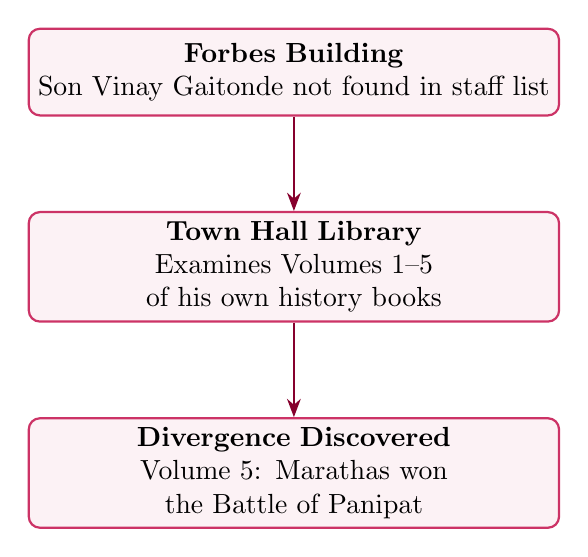
\begin{tikzpicture}[
    node distance=1.2cm,
    block/.style={rectangle, draw=purple!80, fill=purple!5, thick, rounded corners, text width=6.5cm, align=center, minimum height=1.1cm},
    arrow/.style={-Stealth, thick, draw=purple!70!black}
]
    \node[block] (forbes) {\textbf{Forbes Building}\\ Son Vinay Gaitonde not found in staff list};
    \node[block, below=of forbes] (townhall) {\textbf{Town Hall Library}\\ Examines Volumes 1--5 of his own history books};
    \node[block, below=of townhall] (panipat) {\textbf{Divergence Discovered}\\ Volume 5: Marathas won the Battle of Panipat};

    \draw[arrow] (forbes) -- (townhall);
    \draw[arrow] (townhall) -- (panipat);
\end{tikzpicture}
\caption{Page 3: Search for Personal Context \& Discovery of Historical Divergence}
\end{figure}

\end{document}
\documentclass[12pt,a4paper]{article}
\usepackage[utf8]{utf8}
\usepackage[margin=1in]{geometry}
\usepackage{tikz}
\usetikzlibrary{shapes.geometric, arrows.meta, positioning}

\title{\textbf{5. The Adventure}\\[0.3em] \Large Textbook Page 47}
\author{\textbf{Author:} Jayant Narlikar \quad|\quad \textbf{Textbook:} Hornbill (Class 11)}
\date{}

\begin{document}

\maketitle

He turned right along Home Street and entered Forbes building.

"I wish to meet Mr Vinay Gaitonde, please," he said to the English receptionist.

She searched through the telephone list, the staff list and then through the directory of employees of all the branches of the firm. She shook her head and said, "I am afraid I can't find anyone of that name either here or in any of our branches. Are you sure he works here?"

This was a blow, not totally unexpected. If he himself were dead in this world, what guarantee had he that his son would be alive? Indeed, he may not even have been born!

He thanked the girl politely and came out. It was characteristic of him not to worry about where he would stay. His main concern was to make his way to the library of the Asiatic Society to solve the riddle of history. Grabbing a quick lunch at a restaurant, he made his way to the Town Hall.

Yes, to his relief, the Town Hall was there, and it did house the library. He entered the reading room and asked for a list of history books including his own.

His five volumes duly arrived on his table. He started from the beginning. Volume one took the history up to the period of Ashoka, volume two up to Samudragupta, volume three up to Mohammad Ghori and volume four up to the death of Aurangzeb. Up to this period history was as he knew it. The change evidently had occurred in the last volume.

Reading volume five from both ends inwards, Gangadharpant finally converged on the precise moment where history had taken a different turn.

That page in the book described the Battle of Panipat, and it mentioned that the Marathas won it handsomely. Abdali was routed and he was chased back to Kabul by the triumphant Maratha army led by Sadashivrao Bhau and his nephew, the young Vishwasrao.

The book did not go into a blow-by-blow account of the battle itself. Rather, it elaborated in detail its consequences for the power struggle in India. Gangadharpant read through the account avidly. The style of writing was unmistakably his, yet he was reading the account for the first time!

\vfill

\begin{figure}[htbp]
\centering
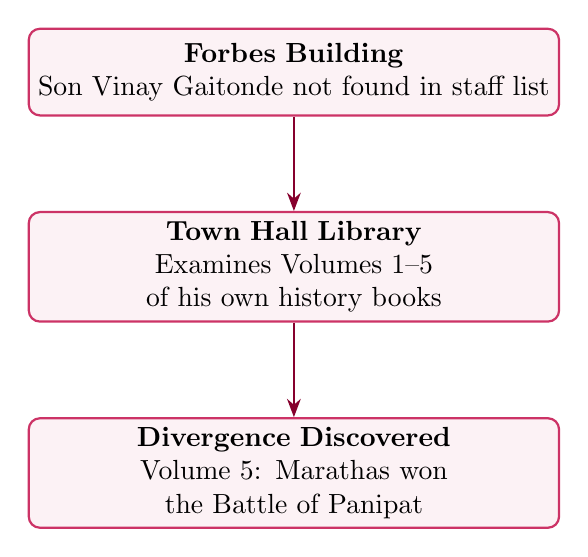
\begin{tikzpicture}[
    node distance=1.2cm,
    block/.style={rectangle, draw=purple!80, fill=purple!5, thick, rounded corners, text width=6.5cm, align=center, minimum height=1.1cm},
    arrow/.style={-Stealth, thick, draw=purple!70!black}
]
    \node[block] (forbes) {\textbf{Forbes Building}\\ Son Vinay Gaitonde not found in staff list};
    \node[block, below=of forbes] (townhall) {\textbf{Town Hall Library}\\ Examines Volumes 1--5 of his own history books};
    \node[block, below=of townhall] (panipat) {\textbf{Divergence Discovered}\\ Volume 5: Marathas won the Battle of Panipat};

    \draw[arrow] (forbes) -- (townhall);
    \draw[arrow] (townhall) -- (panipat);
\end{tikzpicture}
\caption{Page 3: Search for Personal Context \& Discovery of Historical Divergence}
\end{figure}

\end{document}
\documentclass[12pt,a4paper]{article}
\usepackage[utf8]{utf8}
\usepackage[margin=1in]{geometry}
\usepackage{tikz}
\usetikzlibrary{shapes.geometric, arrows.meta, positioning}

\title{\textbf{5. The Adventure}\\[0.3em] \Large Textbook Page 48}
\author{\textbf{Author:} Jayant Narlikar \quad|\quad \textbf{Textbook:} Hornbill (Class 11)}
\date{}

\begin{document}

\maketitle

Their victory in the battle was not only a great morale booster to the Marathas but it also established their supremacy in northern India. The East India Company, which had been watching these developments from the sidelines, got the message and temporarily shelved its expansionist programme.

For the Peshwas the immediate result was an increase in the influence of Bhausaheb and Vishwasrao who eventually succeeded his father in 1780 A.D. The trouble-maker, Dadasaheb, was relegated to the background and he eventually retired from state politics.

To its dismay, the East India Company met its match in the new Maratha ruler, Vishwasrao. He and his brother, Madhavrao, combined political acumen with valour and systematically expanded their influence all over India. The Company was reduced to pockets of influence near Bombay, Calcutta\footnote{Now known as Kolkata} and Madras\footnote{Now known as Chennai}, just like its European rivals, the Portuguese and the French.

For political reasons, the Peshwas kept the puppet Mughal regime alive in Delhi. In the nineteenth century these \textit{de facto} rulers from Pune were astute enough to recognise the importance of the technological age dawning in Europe. They set up their own centres for science and technology. Here, the East India Company saw another opportunity to extend its influence. It offered aid and experts. They were accepted only to make the local centres self-sufficient.

The twentieth century brought about further changes inspired by the West. India moved towards a democracy. By then, the Peshwas had lost their enterprise and they were gradually replaced by democratically elected bodies. The Sultanate at Delhi survived even this transition, largely because it wielded no real influence. The Shahenshah of Delhi was no more than a figurehead to rubber-stamp the 'recommendations' made by the central parliament.

As he read on, Gangadharpant began to appreciate the India he had seen. It was a country that had not been subjected to slavery for the white man; it had learnt to stand on its feet and knew what self-respect was. From a position of strength and for purely commercial reasons, it had allowed the British to retain Bombay as the sole outpost on the subcontinent.

\vfill

\begin{figure}[htbp]
\centering
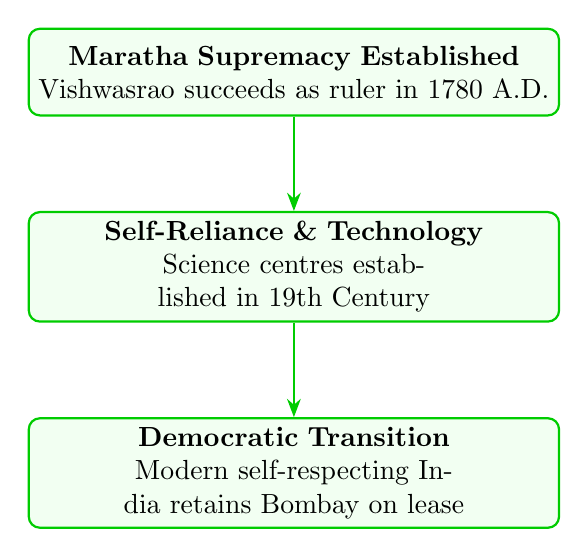
\begin{tikzpicture}[
    node distance=1.2cm,
    block/.style={rectangle, draw=green!80!black, fill=green!5, thick, rounded corners, text width=6.5cm, align=center, minimum height=1.1cm},
    arrow/.style={-Stealth, thick, draw=green!80!black}
]
    \node[block] (maratha) {\textbf{Maratha Supremacy Established}\\ Vishwasrao succeeds as ruler in 1780 A.D.};
    \node[block, below=of maratha] (tech) {\textbf{Self-Reliance \& Technology}\\ Science centres established in 19th Century};
    \node[block, below=of tech] (demo) {\textbf{Democratic Transition}\\ Modern self-respecting India retains Bombay on lease};

    \draw[arrow] (maratha) -- (tech);
    \draw[arrow] (tech) -- (demo);
\end{tikzpicture}
\caption{Page 4: Historical Trajectory of Alternate Sovereign India}
\end{figure}

\end{document}
\documentclass[12pt,a4paper]{article}
\usepackage[utf8]{utf8}
\usepackage[margin=1in]{geometry}
\usepackage{tikz}
\usetikzlibrary{shapes.geometric, arrows.meta, positioning}

\title{\textbf{5. The Adventure}\\[0.3em] \Large Textbook Page 49}
\author{\textbf{Author:} Jayant Narlikar \quad|\quad \textbf{Textbook:} Hornbill (Class 11)}
\date{}

\begin{document}

\maketitle

That lease was to expire in the year 2001, according to a treaty of 1908.

Gangadharpant could not help comparing the country he knew with what he was witnessing around him.

But, at the same time, he felt that his investigations were incomplete. How did the Marathas win the battle? To find the answer he must look for accounts of the battle itself.

He went through the books and journals before him. At last, among the books he found one that gave him the clue. It was \textit{Bhausahebanchi Bakhar}.

Although he seldom relied on the \textit{Bakhars} for historical evidence, he found them entertaining to read. Sometimes, buried in the graphic but doctored accounts, he could spot the germ of truth. He found one now in a three-line account of how close Vishwasrao had come to being killed:

\begin{quotation}
\textit{... And then Vishwasrao guided his horse to the melee where the elite troops were fighting and he attacked them. And God was merciful. A shot brushed past his ear. Even the difference of a til (sesame) would have led to his death.}
\end{quotation}

At eight o'clock the librarian politely reminded the professor that the library was closing for the day. Gangadharpant emerged from his thoughts. Looking around he noticed that he was the only reader left in that magnificent hall.

"I beg your pardon, sir! May I request you to keep these books here for my use tomorrow morning? By the way, when do you open?"

"At eight o'clock, sir." The librarian smiled. Here was a user and researcher right after his heart.

As the professor left the table he shoved some notes into his right pocket. Absent-mindedly, he also shoved the \textit{Bakhar} into his left pocket.

\begin{center}
    * \quad * \quad *
\end{center}

He found a guest house to stay in and had a frugal meal. He then set out for a stroll towards the Azad Maidan.

In the maidan he found a throng moving towards a pandal. So, a lecture was to take place. Force of habit took Professor Gaitonde towards the pandal. The lecture was in progress, although people kept coming and going. But Professor Gaitonde was not looking at the audience. He was staring at the platform as if mesmerised. There was a table and a chair but the latter was unoccupied.

\vfill

\begin{figure}[htbp]
\centering
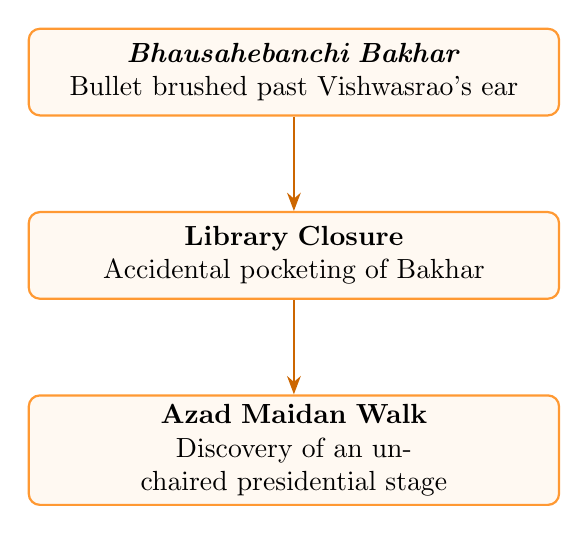
\begin{tikzpicture}[
    node distance=1.2cm,
    block/.style={rectangle, draw=orange!80, fill=orange!5, thick, rounded corners, text width=6.5cm, align=center, minimum height=1.1cm},
    arrow/.style={-Stealth, thick, draw=orange!80!black}
]
    \node[block] (bakhar) {\textbf{\textit{Bhausahebanchi Bakhar}}\\ Bullet brushed past Vishwasrao's ear};
    \node[block, below=of bakhar] (pocket) {\textbf{Library Closure}\\ Accidental pocketing of Bakhar};
    \node[block, below=of pocket] (maidan) {\textbf{Azad Maidan Walk}\\ Discovery of an unchaired presidential stage};

    \draw[arrow] (bakhar) -- (pocket);
    \draw[arrow] (pocket) -- (maidan);
\end{tikzpicture}
\caption{Page 5: Critical Evidence Acquisition \& Azad Maidan Discovery}
\end{figure}

\end{document}
\documentclass[12pt,a4paper]{article}
\usepackage[utf8]{utf8}
\usepackage[margin=1in]{geometry}
\usepackage{tikz}
\usetikzlibrary{shapes.geometric, arrows.meta, positioning}

\title{\textbf{5. The Adventure}\\[0.3em] \Large Textbook Page 49}
\author{\textbf{Author:} Jayant Narlikar \quad|\quad \textbf{Textbook:} Hornbill (Class 11)}
\date{}

\begin{document}

\maketitle

That lease was to expire in the year 2001, according to a treaty of 1908.

Gangadharpant could not help comparing the country he knew with what he was witnessing around him.

But, at the same time, he felt that his investigations were incomplete. How did the Marathas win the battle? To find the answer he must look for accounts of the battle itself.

He went through the books and journals before him. At last, among the books he found one that gave him the clue. It was \textit{Bhausahebanchi Bakhar}.

Although he seldom relied on the \textit{Bakhars} for historical evidence, he found them entertaining to read. Sometimes, buried in the graphic but doctored accounts, he could spot the germ of truth. He found one now in a three-line account of how close Vishwasrao had come to being killed:

\begin{quotation}
\textit{... And then Vishwasrao guided his horse to the melee where the elite troops were fighting and he attacked them. And God was merciful. A shot brushed past his ear. Even the difference of a til (sesame) would have led to his death.}
\end{quotation}

At eight o'clock the librarian politely reminded the professor that the library was closing for the day. Gangadharpant emerged from his thoughts. Looking around he noticed that he was the only reader left in that magnificent hall.

"I beg your pardon, sir! May I request you to keep these books here for my use tomorrow morning? By the way, when do you open?"

"At eight o'clock, sir." The librarian smiled. Here was a user and researcher right after his heart.

As the professor left the table he shoved some notes into his right pocket. Absent-mindedly, he also shoved the \textit{Bakhar} into his left pocket.

\begin{center}
    * \quad * \quad *
\end{center}

He found a guest house to stay in and had a frugal meal. He then set out for a stroll towards the Azad Maidan.

In the maidan he found a throng moving towards a pandal. So, a lecture was to take place. Force of habit took Professor Gaitonde towards the pandal. The lecture was in progress, although people kept coming and going. But Professor Gaitonde was not looking at the audience. He was staring at the platform as if mesmerised. There was a table and a chair but the latter was unoccupied.

\vfill

\begin{figure}[htbp]
\centering
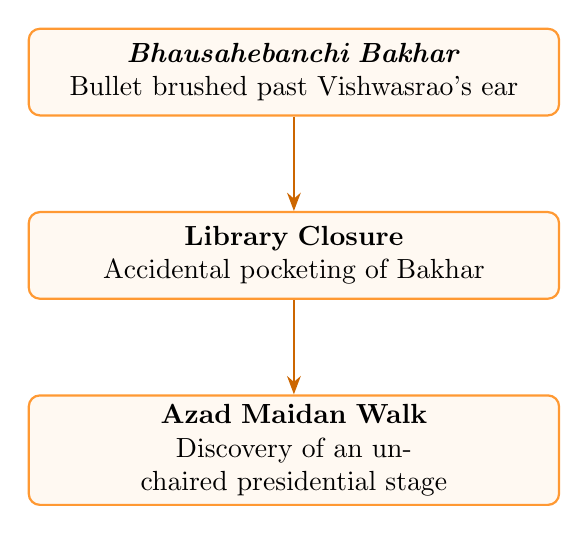
\begin{tikzpicture}[
    node distance=1.2cm,
    block/.style={rectangle, draw=orange!80, fill=orange!5, thick, rounded corners, text width=6.5cm, align=center, minimum height=1.1cm},
    arrow/.style={-Stealth, thick, draw=orange!80!black}
]
    \node[block] (bakhar) {\textbf{\textit{Bhausahebanchi Bakhar}}\\ Bullet brushed past Vishwasrao's ear};
    \node[block, below=of bakhar] (pocket) {\textbf{Library Closure}\\ Accidental pocketing of Bakhar};
    \node[block, below=of pocket] (maidan) {\textbf{Azad Maidan Walk}\\ Discovery of an unchaired presidential stage};

    \draw[arrow] (bakhar) -- (pocket);
    \draw[arrow] (pocket) -- (maidan);
\end{tikzpicture}
\caption{Page 5: Critical Evidence Acquisition \& Azad Maidan Discovery}
\end{figure}

\end{document}
\documentclass[12pt,a4paper]{article}
\usepackage[utf8]{utf8}
\usepackage[margin=1in]{geometry}
\usepackage{tikz}
\usetikzlibrary{shapes.geometric, arrows.meta, positioning}

\title{\textbf{5. The Adventure}\\[0.3em] \Large Textbook Page 50}
\author{\textbf{Author:} Jayant Narlikar \quad|\quad \textbf{Textbook:} Hornbill (Class 11)}
\date{}

\begin{document}

\maketitle

The presidential chair unoccupied! The sight stirred him to the depths. Like a piece of iron attracted to a magnet, he swiftly moved towards the chair.

The speaker stopped in mid-sentence, too shocked to continue. But the audience soon found voice.

"Vacate the chair!"

"This lecture series has no chairperson..."

"Away from the platform, mister!"

"The chair is symbolic, don't you know?"

What nonsense! Whoever heard of a public lecture without a presiding dignitary? Professor Gaitonde went to the mike and gave vent to his views. "Ladies and gentlemen, an unchaired lecture is like Shakespeare's \textit{Hamlet} without the Prince of Denmark. Let me tell you..."

But the audience was in no mood to listen. "Tell us nothing. We are sick of remarks from the chair, of vote of thanks, of long introductions."

"We only want to listen to the speaker..."

"We abolished the old customs long ago..."

"Keep the platform empty, please..."

But Gangadharpant had the experience of speaking at 999 meetings and had faced the Pune audience at its most hostile. He kept on talking.

He soon became a target for a shower of tomatoes, eggs and other objects. But he kept on trying valiantly to correct this sacrilege. Finally, the audience swarmed to the stage to eject him bodily.

And, in the crowd Gangadharpant was nowhere to be seen.

\begin{center}
    * \quad * \quad *
\end{center}

"That is all I have to tell, Rajendra. All I know is that I was found in the Azad Maidan in the morning. But I was back in the world I am familiar with. Now, where exactly did I spend those two days when I was absent from here?"

Rajendra was dumbfounded by the narrative. It took him a while to reply.

"Professor, before, just prior to your collision with the truck, what were you doing?" Rajendra asked.

\vfill

\begin{figure}[htbp]
\centering
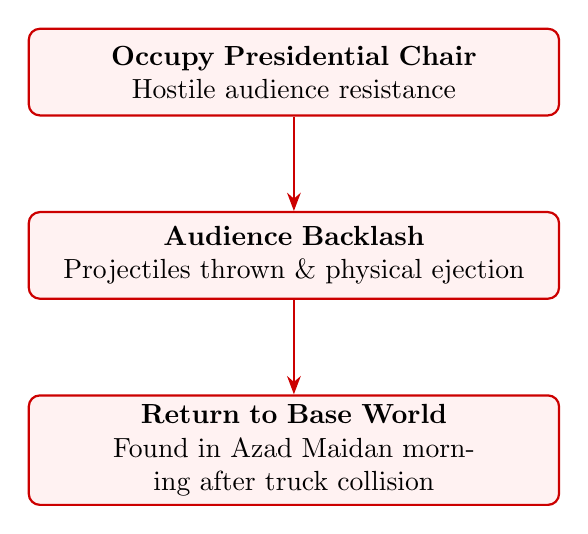
\begin{tikzpicture}[
    node distance=1.2cm,
    block/.style={rectangle, draw=red!80!black, fill=red!5, thick, rounded corners, text width=6.5cm, align=center, minimum height=1.1cm},
    arrow/.style={-Stealth, thick, draw=red!80!black}
]
    \node[block] (stage) {\textbf{Occupy Presidential Chair}\\ Hostile audience resistance};
    \node[block, below=of stage] (eject) {\textbf{Audience Backlash}\\ Projectiles thrown \& physical ejection};
    \node[block, below=of eject] (return) {\textbf{Return to Base World}\\ Found in Azad Maidan morning after truck collision};

    \draw[arrow] (stage) -- (eject);
    \draw[arrow] (eject) -- (return);
\end{tikzpicture}
\caption{Page 6: Azad Maidan Incident \& Return to Original World}
\end{figure}

\end{document}
\documentclass[12pt,a4paper]{article}
\usepackage[utf8]{utf8}
\usepackage[margin=1in]{geometry}
\usepackage{tikz}
\usetikzlibrary{shapes.geometric, arrows.meta, positioning}

\title{\textbf{5. The Adventure}\\[0.3em] \Large Textbook Page 51}
\author{\textbf{Author:} Jayant Narlikar \quad|\quad \textbf{Textbook:} Hornbill (Class 11)}
\date{}

\begin{document}

\maketitle

"I was thinking of the catastrophe theory and its implications for history."

"Right! I thought so!" Rajendra smiled.

"Don't smile smugly. In case you think that it was just my mind playing tricks and my imagination running amok, look at this."

And, triumphantly, Professor Gaitonde produced his vital piece of evidence: a page torn out of a book.

Rajendra read the text on the printed page and his face underwent a change. Gone was the smile and in its place came a grave expression. He was visibly moved.

Gangadharpant pressed home his advantage. "I had inadvertently slipped the \textit{Bakhar} in my pocket as I left the library. I discovered my error when I was paying for my meal. I had intended to return it the next morning. But it seems that in the melee of Azad Maidan, the book was lost; only this torn-off page remained. And, luckily for me, the page contains vital evidence."

Rajendra again read the page. It described how Vishwasrao narrowly missed the bullet; and how that event, taken as an omen by the Maratha army, turned the tide in their favour.

"Now look at this." Gangadharpant produced his own copy of \textit{Bhausahebanchi Bakhar}, opened at the relevant page. The account ran thus:

\begin{quotation}
\textit{... And then Vishwasrao guided his horse to the melee where the elite troops were fighting, and he attacked them. And God expressed His displeasure. He was hit by the bullet.}
\end{quotation}

"Professor Gaitonde, you have given me food for thought. Until I saw this material evidence, I had simply put your experience down to fantasy. But facts can be stranger than fantasies, as I am beginning to realise."

"Facts? What are the facts? I am dying to know!" Professor Gaitonde said.

\begin{center}
    * \quad * \quad *
\end{center}

Rajendra motioned him to silence and started pacing the room, obviously under great mental strain. Finally, he turned around and said, "Professor Gaitonde, I will try to rationalise your experience on the basis of two scientific theories as known today. Whether I succeed or not in convincing you of the facts, only you can judge --- for you have indeed passed through a fantastic experience: or, more correctly, a catastrophic experience!"

\vfill

\begin{figure}[htbp]
\centering
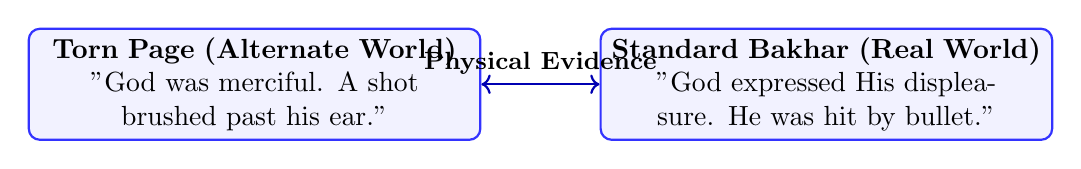
\begin{tikzpicture}[
    box/.style={rectangle, draw=blue!80, fill=blue!5, thick, rounded corners, text width=5.5cm, align=center, minimum height=1.3cm},
    arrow/.style={-Stealth, thick, draw=blue!70!black}
]
    \node[box] (a) {\textbf{Torn Page (Alternate World)}\\ "God was merciful. A shot brushed past his ear."};
    \node[box, right=1.5cm of a] (b) {\textbf{Standard Bakhar (Real World)}\\ "God expressed His displeasure. He was hit by bullet."};

    \draw[arrow, <->] (a) -- node[above, font=\small\bfseries] {Physical Evidence} (b);
\end{tikzpicture}
\caption{Page 7: Comparison of Physical Textual Evidence}
\end{figure}

\end{document}
\documentclass[12pt,a4paper]{article}
\usepackage[utf8]{utf8}
\usepackage[margin=1in]{geometry}
\usepackage{tikz}
\usetikzlibrary{shapes.geometric, arrows.meta, positioning}

\title{\textbf{5. The Adventure}\\[0.3em] \Large Textbook Page 52}
\author{\textbf{Author:} Jayant Narlikar \quad|\quad \textbf{Textbook:} Hornbill (Class 11)}
\date{}

\begin{document}

\maketitle

"Please continue, Rajendra! I am all ears," Professor Gaitonde replied. Rajendra continued pacing as he talked.

"You have heard a lot about the catastrophe theory at that seminar. Let us apply it to the Battle of Panipat. Wars fought face to face on open grounds offer excellent examples of this theory. The Maratha army was facing Abdali's troops on the field of Panipat. There was no great disparity between the latter's troops and the opposing forces. Their armour was comparable. So, a lot depended on the leadership and the morale of the troops. The juncture at which Vishwasrao, the son of and heir to the Peshwa, was killed proved to be the turning point. As history has it, his uncle, Bhausaheb, rushed into the melee and was never seen again. Whether he was killed in battle or survived is not known. But for the troops at that particular moment, that blow of losing their leaders was crucial. They lost their morale and fighting spirit. There followed an utter rout.

"Exactly, Professor! And what you have shown me on that torn page is the course taken by the battle, when the bullet missed Vishwasrao. A crucial event gone the other way. And its effect on the troops was also the opposite. It boosted their morale and provided just that extra impetus that made all the difference," Rajendra said.

"Maybe so. Similar statements are made about the Battle of Waterloo, which Napoleon could have won. But we live in a unique world which has a unique history. This idea of 'it might have been' is okay for the sake of speculation but not for reality," Gangadharpant said.

"I take issue with you there. In fact, that brings me to my second point which you may find strange; but please hear me out," Rajendra said.

Gangadharpant listened expectantly as Rajendra continued. "What do we mean by reality? We experience it directly with our senses or indirectly via instruments. But is it limited to what we see? Does it have other manifestations?

"That reality may not be unique has been found from experiments on very small systems---of atoms and their constituent particles. When dealing with such systems the physicist discovered something startling. The behaviour of these systems cannot be predicted definitively even if all the physical laws governing those systems are known.

"Take an example. I fire an electron from a source. Where will it go? If I fire a bullet from a gun in a given direction at a given speed, I know where it will be at a later time. But I cannot make such an assertion for the electron. It may be here, there, anywhere. I can at best quote odds for it being found in a specified location at a specified time."

\vfill

\begin{figure}[htbp]
\centering
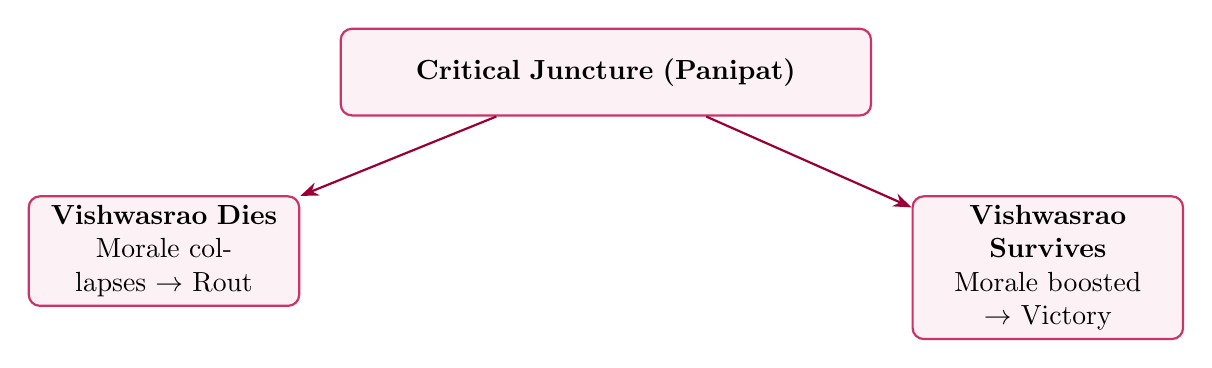
\begin{tikzpicture}[
    node distance=1.2cm,
    block/.style={rectangle, draw=purple!80, fill=purple!5, thick, rounded corners, text width=6.5cm, align=center, minimum height=1.1cm},
    arrow/.style={-Stealth, thick, draw=purple!80!black}
]
    \node[block] (trig) {\textbf{Critical Juncture (Panipat)}};
    \node[block, below left=1cm and 0.5cm of trig, text width=3.2cm] (patha) {\textbf{Vishwasrao Dies}\\ Morale collapses $\rightarrow$ Rout};
    \node[block, below right=1cm and 0.5cm of trig, text width=3.2cm] (pathb) {\textbf{Vishwasrao Survives}\\ Morale boosted $\rightarrow$ Victory};

    \draw[arrow] (trig) -- (patha);
    \draw[arrow] (trig) -- (pathb);
\end{tikzpicture}
\caption{Page 8: Application of Catastrophe Theory to Panipat}
\end{figure}

\end{document}
\documentclass[12pt,a4paper]{article}
\usepackage[utf8]{utf8}
\usepackage[margin=1in]{geometry}
\usepackage{tikz}
\usetikzlibrary{shapes.geometric, arrows.meta, positioning}

\title{\textbf{5. The Adventure}\\[0.3em] \Large Textbook Page 53}
\author{\textbf{Author:} Jayant Narlikar \quad|\quad \textbf{Textbook:} Hornbill (Class 11)}
\date{}

\begin{document}

\maketitle

"The lack of determinism in quantum theory! Even an ignoramus historian like me has heard of it," Professor Gaitonde said.

"So, imagine many world pictures. In one world the electron is found here, in another it is over there. In yet another it is in a still different location. Once the observer finds where it is, we know which world we are talking about. But all those alternative worlds could exist just the same." Rajendra paused to marshall his thoughts.

"But is there any contact between those many worlds?" Professor Gaitonde asked.

"Yes and no! Imagine two worlds, for example. In both an electron is orbiting the nucleus of an atom..."

"Like planets around the sun..." Gangadharpant interjected.

"Not quite. We know the precise trajectory of the planet. The electron could be orbiting in any of a large number of specified states. These states may be used to identify the world. In state no. 1 we have the electron in a state of higher energy. In state no. 2 it is in a state of lower energy. It can make a jump from high to low energy and send out a pulse of radiation. Or a pulse of radiation can knock it out of state no. 2 into state no. 1. Such transitions are common in microscopic systems. What if it happened on a macroscopic level?" Rajendra said.

"I get you! You are suggesting that I made a transition from one world to another and back again?" Gangadharpant asked.

"Fantastic though it seems, this is the only explanation I can offer. My theory is that catastrophic situations offer radically different alternatives for the world to proceed. It seems that so far as reality is concerned all alternatives are viable but the observer can experience only one of them at a time.

"By making a transition, you were able to experience two worlds although one at a time. The one you live in now and the one where you spent two days. One has the history we know, the other a different history. The separation or bifurcation took place in the Battle of Panipat. You neither travelled to the past nor to the future. You were in the present but experiencing a different world. Of course, by the same token there must be many more different worlds arising out of bifurcations at different points of time."

\vfill

\begin{figure}[htbp]
\centering
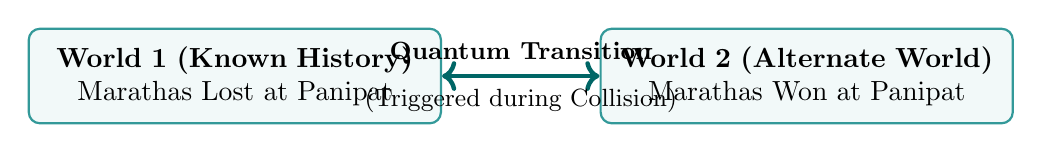
\begin{tikzpicture}[
    node distance=1.5cm,
    world/.style={rectangle, draw=teal!80, fill=teal!5, thick, rounded corners, text width=5cm, align=center, minimum height=1.2cm},
    arrow/.style={-Stealth, ultra thick, draw=teal!80!black}
]
    \node[world] (w1) {\textbf{World 1 (Known History)}\\ Marathas Lost at Panipat};
    \node[world, right=2cm of w1] (w2) {\textbf{World 2 (Alternate World)}\\ Marathas Won at Panipat};

    \draw[arrow, <->] (w1) -- node[above, font=\small\bfseries] {Quantum Transition} node[below, font=\small] {(Triggered during Collision)} (w2);
\end{tikzpicture}
\caption{Page 9: Quantum Transition Between Parallel World Realities}
\end{figure}

\end{document}
\documentclass[12pt,a4paper]{article}
\usepackage[utf8]{utf8}
\usepackage[margin=1in]{geometry}
\usepackage{tikz}
\usetikzlibrary{shapes.geometric, arrows.meta, positioning}

\title{\textbf{5. The Adventure}\\[0.3em] \Large Textbook Page 54}
\author{\textbf{Author:} Jayant Narlikar \quad|\quad \textbf{Textbook:} Hornbill (Class 11)}
\date{}

\begin{document}

\maketitle

As Rajendra concluded, Gangadharpant asked the question that was beginning to bother him most. "But why did I make the transition?"

"If I knew the answer I would solve a great problem. Unfortunately, there are many unsolved questions in science and this is one of them. But that does not stop me from guessing." Rajendra smiled and proceeded, "You need some interaction to cause a transition. Perhaps, at the time of the collision you were thinking about the catastrophe theory and its role in wars. Maybe you were wondering about the Battle of Panipat. Perhaps, the neurons in your brain acted as a trigger."

"A good guess. I was indeed wondering what course history would have taken if the result of the battle had gone the other way," Professor Gaitonde said. "That was going to be the topic of my thousandth presidential address."

"Now you are in the happy position of recounting your real life experience rather than just speculating," Rajendra laughed.

But Gangadharpant was grave.

"No, Rajendra, my thousandth address was made on the Azad Maidan when I was so rudely interrupted. No. The Professor Gaitonde who disappeared while defending his chair on the platform will now never be seen presiding at another meeting --- I have conveyed my regrets to the organisers of the Panipat seminar."

\section*{Understanding the text}
\subsection*{I. Tick the statements that are true.}
\begin{enumerate}
    \item The story is an account of real events.
    \item The story hinges on a particular historical event.
    \item Rajendra Deshpande was a historian.
    \item The places mentioned in the story are all imaginary.
    \item The story tries to relate history to science.
\end{enumerate}

\subsection*{II. Briefly explain the following statements from the text.}
\begin{enumerate}
    \item "You neither travelled to the past nor the future. You were in the present experiencing a different world."
    \item "You have passed through a fantastic experience: or more correctly, a catastrophic experience."
    \item Gangadharpant could not help comparing the country he knew with what he was witnessing around him.
\end{enumerate}

\vfill

\begin{figure}[htbp]
\centering
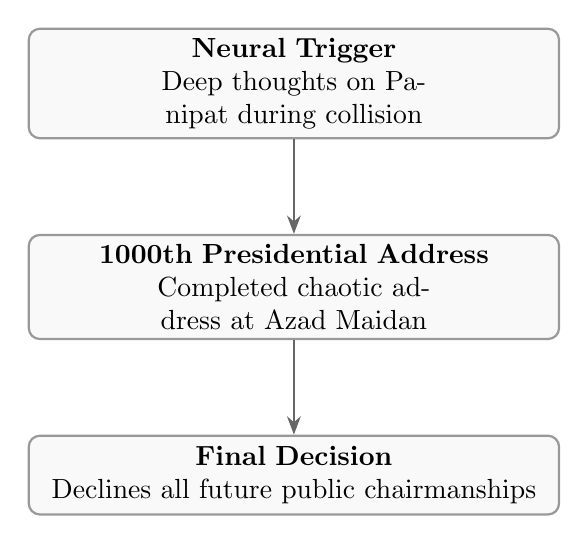
\begin{tikzpicture}[
    node distance=1.2cm,
    block/.style={rectangle, draw=gray!80, fill=gray!5, thick, rounded corners, text width=6.5cm, align=center, minimum height=1cm},
    arrow/.style={-Stealth, thick, draw=gray!80!black}
]
    \node[block] (thought) {\textbf{Neural Trigger}\\ Deep thoughts on Panipat during collision};
    \node[block, below=of thought] (address) {\textbf{1000th Presidential Address}\\ Completed chaotic address at Azad Maidan};
    \node[block, below=of address] (refusal) {\textbf{Final Decision}\\ Declines all future public chairmanships};

    \draw[arrow] (thought) -- (address);
    \draw[arrow] (address) -- (refusal);
\end{tikzpicture}
\caption{Page 10: Conclusion of Story \& Gaitonde's Decision}
\end{figure}

\end{document}
\documentclass[12pt,a4paper]{article}
\usepackage[utf8]{utf8}
\usepackage[margin=1in]{geometry}
\usepackage{tikz}
\usetikzlibrary{shapes.geometric, arrows.meta, positioning}

\title{\textbf{Exercises \& Discussions}\\[0.3em] \Large Textbook Page 55}
\author{\textbf{Textbook:} Hornbill (Class 11)}
\date{}

\begin{document}

\maketitle

\begin{enumerate}
    \item[4.] "The lack of determinism in quantum theory!"
    \item[5.] "You need some interaction to cause a transition."
\end{enumerate}

\section*{Talking about the text}
\begin{enumerate}
    \item Discuss the following statements in groups of two pairs, each pair in a group taking opposite points of view.
    \begin{enumerate}
        \item A single event may change the course of the history of a nation.
        \item Reality is what is directly experienced through the senses.
        \item The methods of inquiry of history, science and philosophy are similar.
    \end{enumerate}
    \item 
    \begin{enumerate}
        \item The story is called 'The Adventure'. Compare it with the adventure described in 'We're Not Afraid to Die...'
        \item Why do you think Professor Gaitonde decided never to preside over meetings again?
    \end{enumerate}
\end{enumerate}

\section*{Thinking about language}
\begin{enumerate}
    \item In which language do you think Gangadharpant and Khan Sahib talked to each other? Which language did Gangadharpant use to talk to the English receptionist?
    \item In which language do you think \textit{Bhausahebanchi Bakhar} was written?
    \item There is mention of three communities in the story: the Marathas, the Mughals, the Anglo-Indians. Which language do you think they used within their communities and while speaking to the other groups?
    \item Do you think that the ruled always adopt the language of the ruler?
\end{enumerate}

\section*{Working with words}
\subsection*{I. Tick the item that is closest in meaning to the following phrases.}
\begin{enumerate}
    \item \textbf{to take issue with}: (i) to accept \quad (ii) to discuss \quad (iii) to disagree \quad (iv) to add
\end{enumerate}

\vfill

\begin{figure}[htbp]
\centering
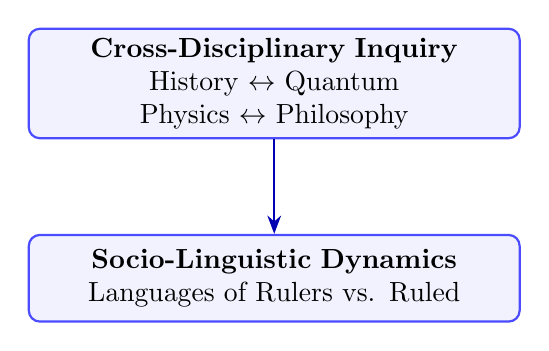
\begin{tikzpicture}[
    node distance=1.2cm,
    block/.style={rectangle, draw=blue!70, fill=blue!5, thick, rounded corners, text width=6cm, align=center, minimum height=1.1cm},
    arrow/.style={-Stealth, thick, draw=blue!70!black}
]
    \node[block] (disc) {\textbf{Cross-Disciplinary Inquiry}\\ History $\leftrightarrow$ Quantum Physics $\leftrightarrow$ Philosophy};
    \node[block, below=of disc] (lang) {\textbf{Socio-Linguistic Dynamics}\\ Languages of Rulers vs. Ruled};

    \draw[arrow] (disc) -- (lang);
\end{tikzpicture}
\caption{Page 11: Interdisciplinary & Language Exercise Framework}
\end{figure}

\end{document}
\documentclass[12pt,a4paper]{article}
\usepackage[utf8]{utf8}
\usepackage[margin=1in]{geometry}
\usepackage{tikz}
\usetikzlibrary{shapes.geometric, arrows.meta, positioning}

\title{\textbf{Working with Words}\\[0.3em] \Large Textbook Page 56}
\author{\textbf{Textbook:} Hornbill (Class 11)}
\date{}

\begin{document}

\maketitle

\begin{enumerate}
    \item[2.] \textbf{to give vent to}: (i) to express \quad (ii) to emphasise \quad (iii) suppress \quad (iv) dismiss
    \item[3.] \textbf{to stand on one's feet}: (i) to be physically strong \quad (ii) to be independent \quad (iii) to stand erect \quad (iv) to be successful
    \item[4.] \textbf{to be wound up}: (i) to become active \quad (ii) to stop operating \quad (iii) to be transformed \quad (iv) to be destroyed
    \item[5.] \textbf{to meet one's match}: (i) to meet a partner who has similar tastes \quad (ii) to meet an opponent \quad (iii) to meet someone who is equally able as oneself \quad (iv) to meet defeat
\end{enumerate}

\subsection*{II. Distinguish between the following pairs of sentences.}
\begin{enumerate}
    \item 
    \begin{enumerate}
        \item He was visibly moved.
        \item He was visually impaired.
    \end{enumerate}
    \item 
    \begin{enumerate}
        \item Green and black stripes were used alternately.
        \item Green stripes could be used or alternatively black ones.
    \end{enumerate}
    \item 
    \begin{enumerate}
        \item The team played the two matches successfully.
        \item The team played two matches successively.
    \end{enumerate}
    \item 
    \begin{enumerate}
        \item The librarian spoke respectfully to the learned scholar.
        \item You will find the historian and the scientist in the archaeology and natural science sections of the museum respectively.
    \end{enumerate}
\end{enumerate}

\vfill

\begin{figure}[htbp]
\centering
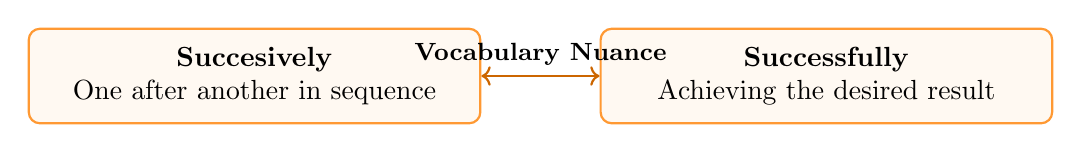
\begin{tikzpicture}[
    box/.style={rectangle, draw=orange!80, fill=orange!5, thick, rounded corners, text width=5.5cm, align=center, minimum height=1.2cm},
    arrow/.style={-Stealth, thick, draw=orange!80!black}
]
    \node[box] (a) {\textbf{Succesively}\\ One after another in sequence};
    \node[box, right=1.5cm of a] (b) {\textbf{Successfully}\\ Achieving the desired result};

    \draw[arrow, <->] (a) -- node[above, font=\small\bfseries] {Vocabulary Nuance} (b);
\end{tikzpicture}
\caption{Page 12: Vocabulary Distinction Analysis}
\end{figure}

\end{document}
\documentclass[12pt,a4paper]{article}
\usepackage[utf8]{utf8}
\usepackage[margin=1in]{geometry}
\usepackage{tcolorbox}
\usepackage{tikz}
\usetikzlibrary{shapes.geometric, arrows.meta, positioning}

\title{\textbf{Noticing Form \& Catastrophe Theory}\\[0.3em] \Large Textbook Page 57}
\author{\textbf{Textbook:} Hornbill (Class 11)}
\date{}

\begin{document}

\maketitle

\section*{Noticing form}
The story deals with unreal and hypothetical conditions. Some of the sentences used to express this notion are given below:
\begin{enumerate}
    \item If I fire a bullet from a gun in a given direction at a given speed, I know where it will be at a later time.
    \item If I knew the answer I would solve a great problem.
    \item If he himself were dead in this world, what guarantee had he that his son would be alive.
    \item What course would history have taken if the battle had gone the other way?
\end{enumerate}
\textit{Notice that in an unreal condition, it is clearly expected that the condition will not be fulfilled.}

\section*{Things to do}
\subsection*{I. Catastrophe Theory Passage}
\begin{tcolorbox}[colback=blue!5!white,colframe=blue!75!black]
Originated by the French mathematician, René Thom, in the 1960s, catastrophe theory is a special branch of dynamical systems theory. It studies and classifies phenomena characterised by sudden shifts in behaviour arising from small changes in circumstances.

Catastrophes are bifurcations between different equilibria, or fixed point attractors. Due to their restricted nature, catastrophes can be classified on the basis of how many control parameters are being simultaneously varied. For example, if there are two controls, then one finds the most common type, called a 'cusp' catastrophe. If, however, there are more than five controls, there is no classification.

Catastrophe theory has been applied to a number of different phenomena, such as the stability of ships at sea and their capsizing, bridge collapse, and, with some less convincing success, the fight-or-flight behaviour of animals and prison riots.
\end{tcolorbox}

\vfill

\begin{figure}[htbp]
\centering
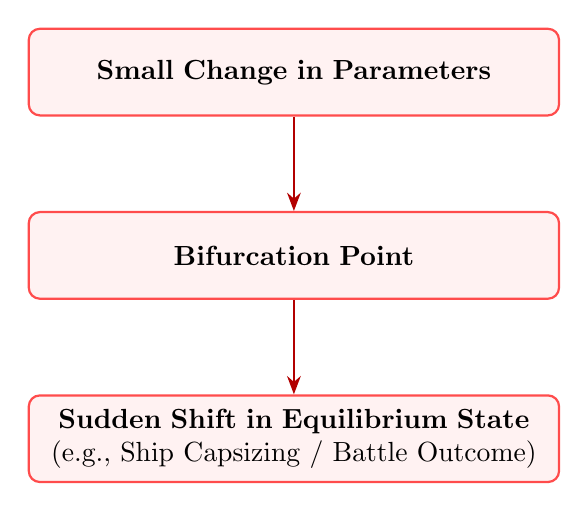
\begin{tikzpicture}[
    node distance=1.2cm,
    block/.style={rectangle, draw=red!70, fill=red!5, thick, rounded corners, text width=6.5cm, align=center, minimum height=1.1cm},
    arrow/.style={-Stealth, thick, draw=red!70!black}
]
    \node[block] (param) {\textbf{Small Change in Parameters}};
    \node[block, below=of param] (bif) {\textbf{Bifurcation Point}};
    \node[block, below=of bif] (shift) {\textbf{Sudden Shift in Equilibrium State}\\ (e.g., Ship Capsizing / Battle Outcome)};

    \draw[arrow] (param) -- (bif);
    \draw[arrow] (bif) -- (shift);
\end{tikzpicture}
\caption{Page 13: Mathematical Model of René Thom's Catastrophe Theory}
\end{figure}

\end{document}
\documentclass[12pt,a4paper]{article}
\usepackage[utf8]{utf8}
\usepackage[margin=1in]{geometry}
\usepackage{tikz}
\usetikzlibrary{shapes.geometric, arrows.meta, positioning}

\title{\textbf{Scientific Theories \& Pedagogical Notes}\\[0.3em] \Large Textbook Page 58}
\author{\textbf{Textbook:} Hornbill (Class 11)}
\date{}

\begin{document}

\maketitle

\subsection*{II. Web / Encyclopedia Research}
Look up the Internet or an encyclopedia for information on the following theories:
\begin{enumerate}
    \item[(i)] Quantum theory
    \item[(ii)] Theory of relativity
    \item[(iii)] Big Bang theory
    \item[(iv)] Theory of evolution
\end{enumerate}

\section*{Notes}
\begin{itemize}
    \item \textbf{Understanding the text:} True/false items to check inferential comprehension; Explaining statements from the text.
    \item \textbf{Talking about the text:} Discussing approaches of various disciplines to knowledge (across the curriculum); Cross-text reference.
    \item \textbf{Thinking about language:} Inter-community communication through common languages; Political domination and language imposition (discuss).
    \item \textbf{Working with words:} Distinguishing between frequently misused word forms: \textit{respectively} / \textit{respectfully}.
    \item \textbf{Noticing form:} Conditional sentences for unreal and hypothetical conditions.
    \item \textbf{Things to do:} Finding out about popular scientific theories (real-life reading).
\end{itemize}

\vfill

\begin{figure}[htbp]
\centering
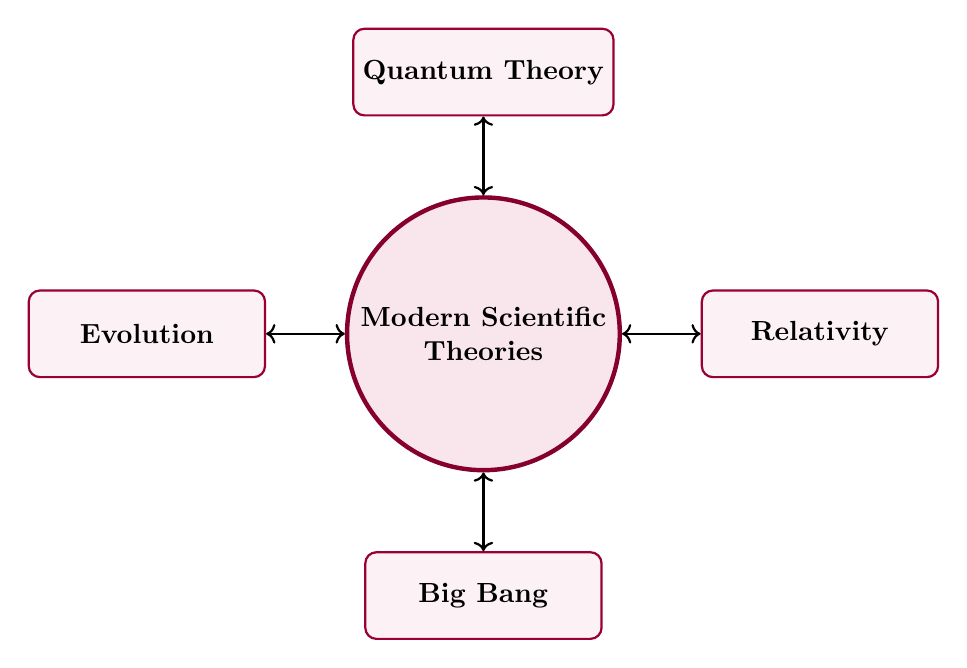
\begin{tikzpicture}[
    center/.style={circle, draw=purple!70!black, fill=purple!10, ultra thick, minimum size=2.8cm, align=center},
    sys/.style={rectangle, draw=purple!80!black, fill=purple!5, thick, rounded corners, minimum width=3cm, minimum height=1.1cm, align=center}
]
    \node[center] (core) {\textbf{Modern Scientific}\\ \textbf{Theories}};
    \node[sys, above=1cm of core] (quant) {\textbf{Quantum Theory}};
    \node[sys, right=1cm of core] (rel) {\textbf{Relativity}};
    \node[sys, below=1cm of core] (bb) {\textbf{Big Bang}};
    \node[sys, left=1cm of core] (evo) {\textbf{Evolution}};

    \draw[<->, thick] (core) -- (quant);
    \draw[<->, thick] (core) -- (rel);
    \draw[<->, thick] (core) -- (bb);
    \draw[<->, thick] (core) -- (evo);
\end{tikzpicture}
\caption{Page 14: Core Pillars of Modern Scientific Theories}
\end{figure}

\end{document}

